% \begin{center}
%     \textbf{\MakeUppercase{Lời mở đầu}}
% \end{center}
% \chapter*{LỜI MỞ ĐẦU}
% \addcontentsline{toc}{chapter}{Lời mở đầu}



\section*{1. Lý do chọn đề tài}
Trong bối cảnh đô thị hóa diễn ra mạnh mẽ, số lượng phương tiện giao thông cá nhân ngày càng gia tăng, đặc biệt là tại các thành phố lớn. Việc quản lý bãi đỗ xe theo phương thức thủ công hiện nay còn tồn tại nhiều hạn chế như mất nhiều thời gian cho việc kiểm soát xe ra vào, khó khăn trong việc thống kê số lượng xe, dễ xảy ra sai sót và gian lận, đồng thời gây ùn tắc tại khu vực cổng bãi xe vào giờ cao điểm.

Để đánh giá thực trạng quản lý bãi đỗ xe và nhu cầu sử dụng dịch vụ giữ xe thông minh, em thực hiện đã tiến hành khảo sát 151 người dùng tại khu vực thành phố Hồ Chí Minh. Kết quả khảo sát được thể hiện qua các biểu đồ sau:

\begin{figure}[H]
    \centering
    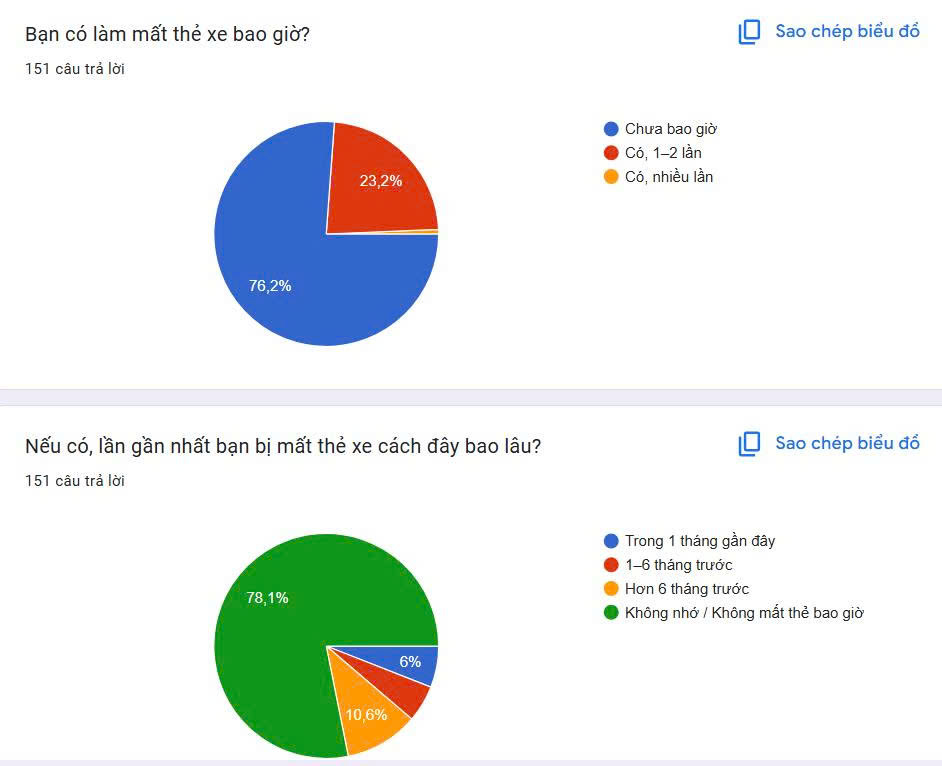
\includegraphics[width=0.9\textwidth]{figures/mat_the.jpg}
    \caption{Kết quả khảo sát về tình trạng mất thẻ xe}
    \label{fig:khaosat1}
\end{figure}

Kết quả cho thấy 76,2\% người tham gia chưa từng bị mất thẻ xe, trong khi 23,2\% đã có trải nghiệm mất thẻ từ 1-2 lần. Đặc biệt, trong số những người từng bị mất thẻ, 78,1\% không nhớ hoặc không có thẻ bảo giờ, điều này cho thấy sự bất tiện lớn của hệ thống thẻ từ truyền thống.

\begin{figure}[H]
    \centering
    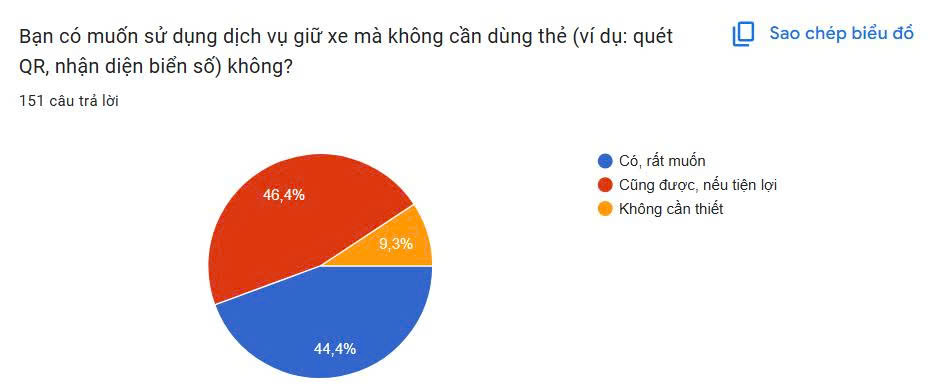
\includegraphics[width=0.9\textwidth]{figures/doi_dv.jpg}
    \caption{Kết quả khảo sát về nhu cầu sử dụng dịch vụ không cần thẻ}
    \label{fig:khaosat2}
\end{figure}
Về nhu cầu sử dụng công nghệ hiện đại, 44,4\% người được hỏi cho biết muốn sử dụng dịch vụ giữ xe không cần thẻ truyền thống , 46,4\% cũng đồng ý nếu tiện lợi hơn và chỉ 9,3\% cho rằng không cần thiết. Điều này chứng tỏ có nhu cầu thực tế cao (90,7\%) đối với giải pháp quản lý bãi đỗ xe thông minh.


Bên cạnh đó, sự phát triển mạnh mẽ của trí tuệ nhân tạo đã mở ra nhiều hướng tiếp cận mới trong việc xây dựng các hệ thống quản lý thông minh. Việc ứng dụng các công nghệ này vào quản lý bãi đỗ xe không chỉ giúp tự động hóa quy trình vận hành mà còn nâng cao hiệu quả quản lý, giảm chi phí nhân lực và cải thiện trải nghiệm người sử dụng.

Xuất phát từ những vấn đề thực tiễn và kết quả khảo sát nêu trên, đề tài Xây dựng hệ thống quản lý bãi đỗ xe thông minh được lựa chọn nhằm nghiên cứu và xây dựng một giải pháp ứng dụng công nghệ hiện đại vào công tác quản lý bãi đỗ xe, loại bỏ sự phụ thuộc vào thẻ từ vật lý, góp phần nâng cao hiệu quả khai thác và vận hành hệ thống.

\section*{2. Tình hình nghiên cứu}
Trong những năm gần đây, nhiều hệ thống quản lý bãi đỗ xe thông minh đã được triển khai sử dụng thẻ từ, mã QR, camera nhận diện biển số và cảm biến phát hiện chỗ trống.

Tại Việt Nam, phần lớn bãi đỗ xe vẫn dùng thẻ từ truyền thống. Theo khảo sát của em thực hiện với 151 người dùng, 23,2\% đã từng mất thẻ xe, trong đó 78,1\% không nhớ hoặc không còn thẻ khi cần lấy xe. Điều này cho thấy hệ thống thẻ từ còn nhiều bất cập.

Một số giải pháp công nghệ cao đã được áp dụng như mã QR hoặc camera nhận diện biển số, nhưng vẫn còn hạn chế về chi phí, khả năng mở rộng và chưa tận dụng triệt để trí tuệ nhân tạo, học sâu cùng điện toán đám mây.

Khảo sát cho thấy 90,7\% người dùng có nhu cầu sử dụng dịch vụ giữ xe không cần thẻ vật lý, chứng tỏ thị trường có tiềm năng lớn cho giải pháp quản lý bãi đỗ xe thông minh.

Do đó, việc xây dựng hệ thống quản lý bãi đỗ xe thông minh sử dụng công nghệ nhận diện biển số và khuôn mặt với chi phí hợp lý là cần thiết và có ý nghĩa thực tiễn tại Việt Nam.
\section*{4. Nhiệm vụ nghiên cứu}
Để đạt được mục tiêu đề ra, đề tài tập trung thực hiện các nhiệm vụ sau:
\begin{itemize}
    \item Khảo sát và phân tích thực trạng quản lý bãi đỗ xe hiện nay.
    \item Nghiên cứu các công nghệ và giải pháp liên quan đến hệ thống quản lý bãi đỗ xe thông minh.
    \item Phân tích yêu cầu chức năng và phi chức năng của hệ thống.
    \item Thiết kế kiến trúc tổng thể, cơ sở dữ liệu và giao diện hệ thống.
    \item Xây dựng và cài đặt hệ thống quản lý bãi đỗ xe thông minh.
    \item Thực hiện kiểm thử và đánh giá kết quả đạt được của hệ thống.
\end{itemize}

\section*{5. Phương pháp nghiên cứu}
Trong quá trình thực hiện đề tài, các phương pháp nghiên cứu sau được sử dụng:
\begin{itemize}
    \item Phương pháp nghiên cứu tài liệu: Thu thập, phân tích các tài liệu, bài báo khoa học và các hệ thống liên quan đến quản lý bãi đỗ xe.
    \item Phương pháp phân tích và thiết kế hệ thống: Phân tích yêu cầu, xây dựng mô hình hệ thống và các sơ đồ UML.
    \item Phương pháp thực nghiệm: Triển khai cài đặt hệ thống, kiểm thử các chức năng và đánh giá hiệu quả hoạt động.
\end{itemize}

\section*{5. Các kết quả đạt được}
Kết quả của đề tài là xây dựng được một hệ thống quản lý bãi đỗ xe thông minh đáp ứng các yêu cầu đề ra. Hệ thống cho phép quản lý xe ra vào một cách tự động, lưu trữ và xử lý dữ liệu chính xác, hỗ trợ giám sát, thống kê và báo cáo tình trạng bãi đỗ xe.

Ngoài ra, đề tài giúp em củng cố và vận dụng kiến thức đã học về lập trình và phân tích thiết kế hệ thống vào thực tế, đồng thời nâng cao kỹ năng nghiên cứu, triển khai và làm việc với các công nghệ mới.
\section*{6. Kết cấu của TTTN}
Bố cục của TTTN được tổ chức thành 5 chương như sau:
\begin{itemize}
    \item \textbf{Chương 1: Cơ sở lý thuyết} - Trình bày các khái niệm, công nghệ và phương pháp liên quan đến hệ thống quản lý bãi đỗ xe thông minh.
    \item \textbf{Chương 2: Phân tích và thiết kế và xây dựng hệ thống} - Phân tích yêu cầu, thiết kế kiến trúc hệ thống và giao diện người dùng.
    \item \textbf{Chương 3: Cài đặt và kiểm thử} - Mô tả quá trình cài đặt, cấu hình và triển khai hệ thống quản lý bãi đỗ xe thông minh.
    \item \textbf{Chương 4: Kết luận và hướng phát triển} - Tổng kết kết quả đạt được, đánh giá hiệu quả của hệ thống và đề xuất hướng phát triển trong tương lai.
\end{itemize}